\documentclass[popl.tex]{subfiles}
\begin{document}

\section{Levenshtein topology and matrices}

These are useful for visually checking different implementations.

\begin{figure}[H]
\begin{center}
\adjustbox{valign=m}{
\includegraphics[width=4cm]{figures/lev_nfa_6x1.pdf}}
\adjustbox{valign=m}{\resizebox{0.4\textwidth}{!}{\input{figures/lev_nfa_6x1}}}
\end{center}
\caption{Lev(|\sigma|=6, \Delta=1) automaton, adjacency and reachability matrix.}
\end{figure}

\begin{figure}[H]
\begin{center}
\adjustbox{valign=m}{
\includegraphics[width=4cm]{figures/lev_nfa_6x2.pdf}}
\adjustbox{valign=m}{\resizebox{0.4\textwidth}{!}{\input{figures/lev_nfa_6x2}}}
\end{center}
\caption{Lev(|\sigma|=6, \Delta=2) automaton, adjacency and reachability matrix.}
\end{figure}

\begin{figure}[H]
\begin{center}
\adjustbox{valign=m}{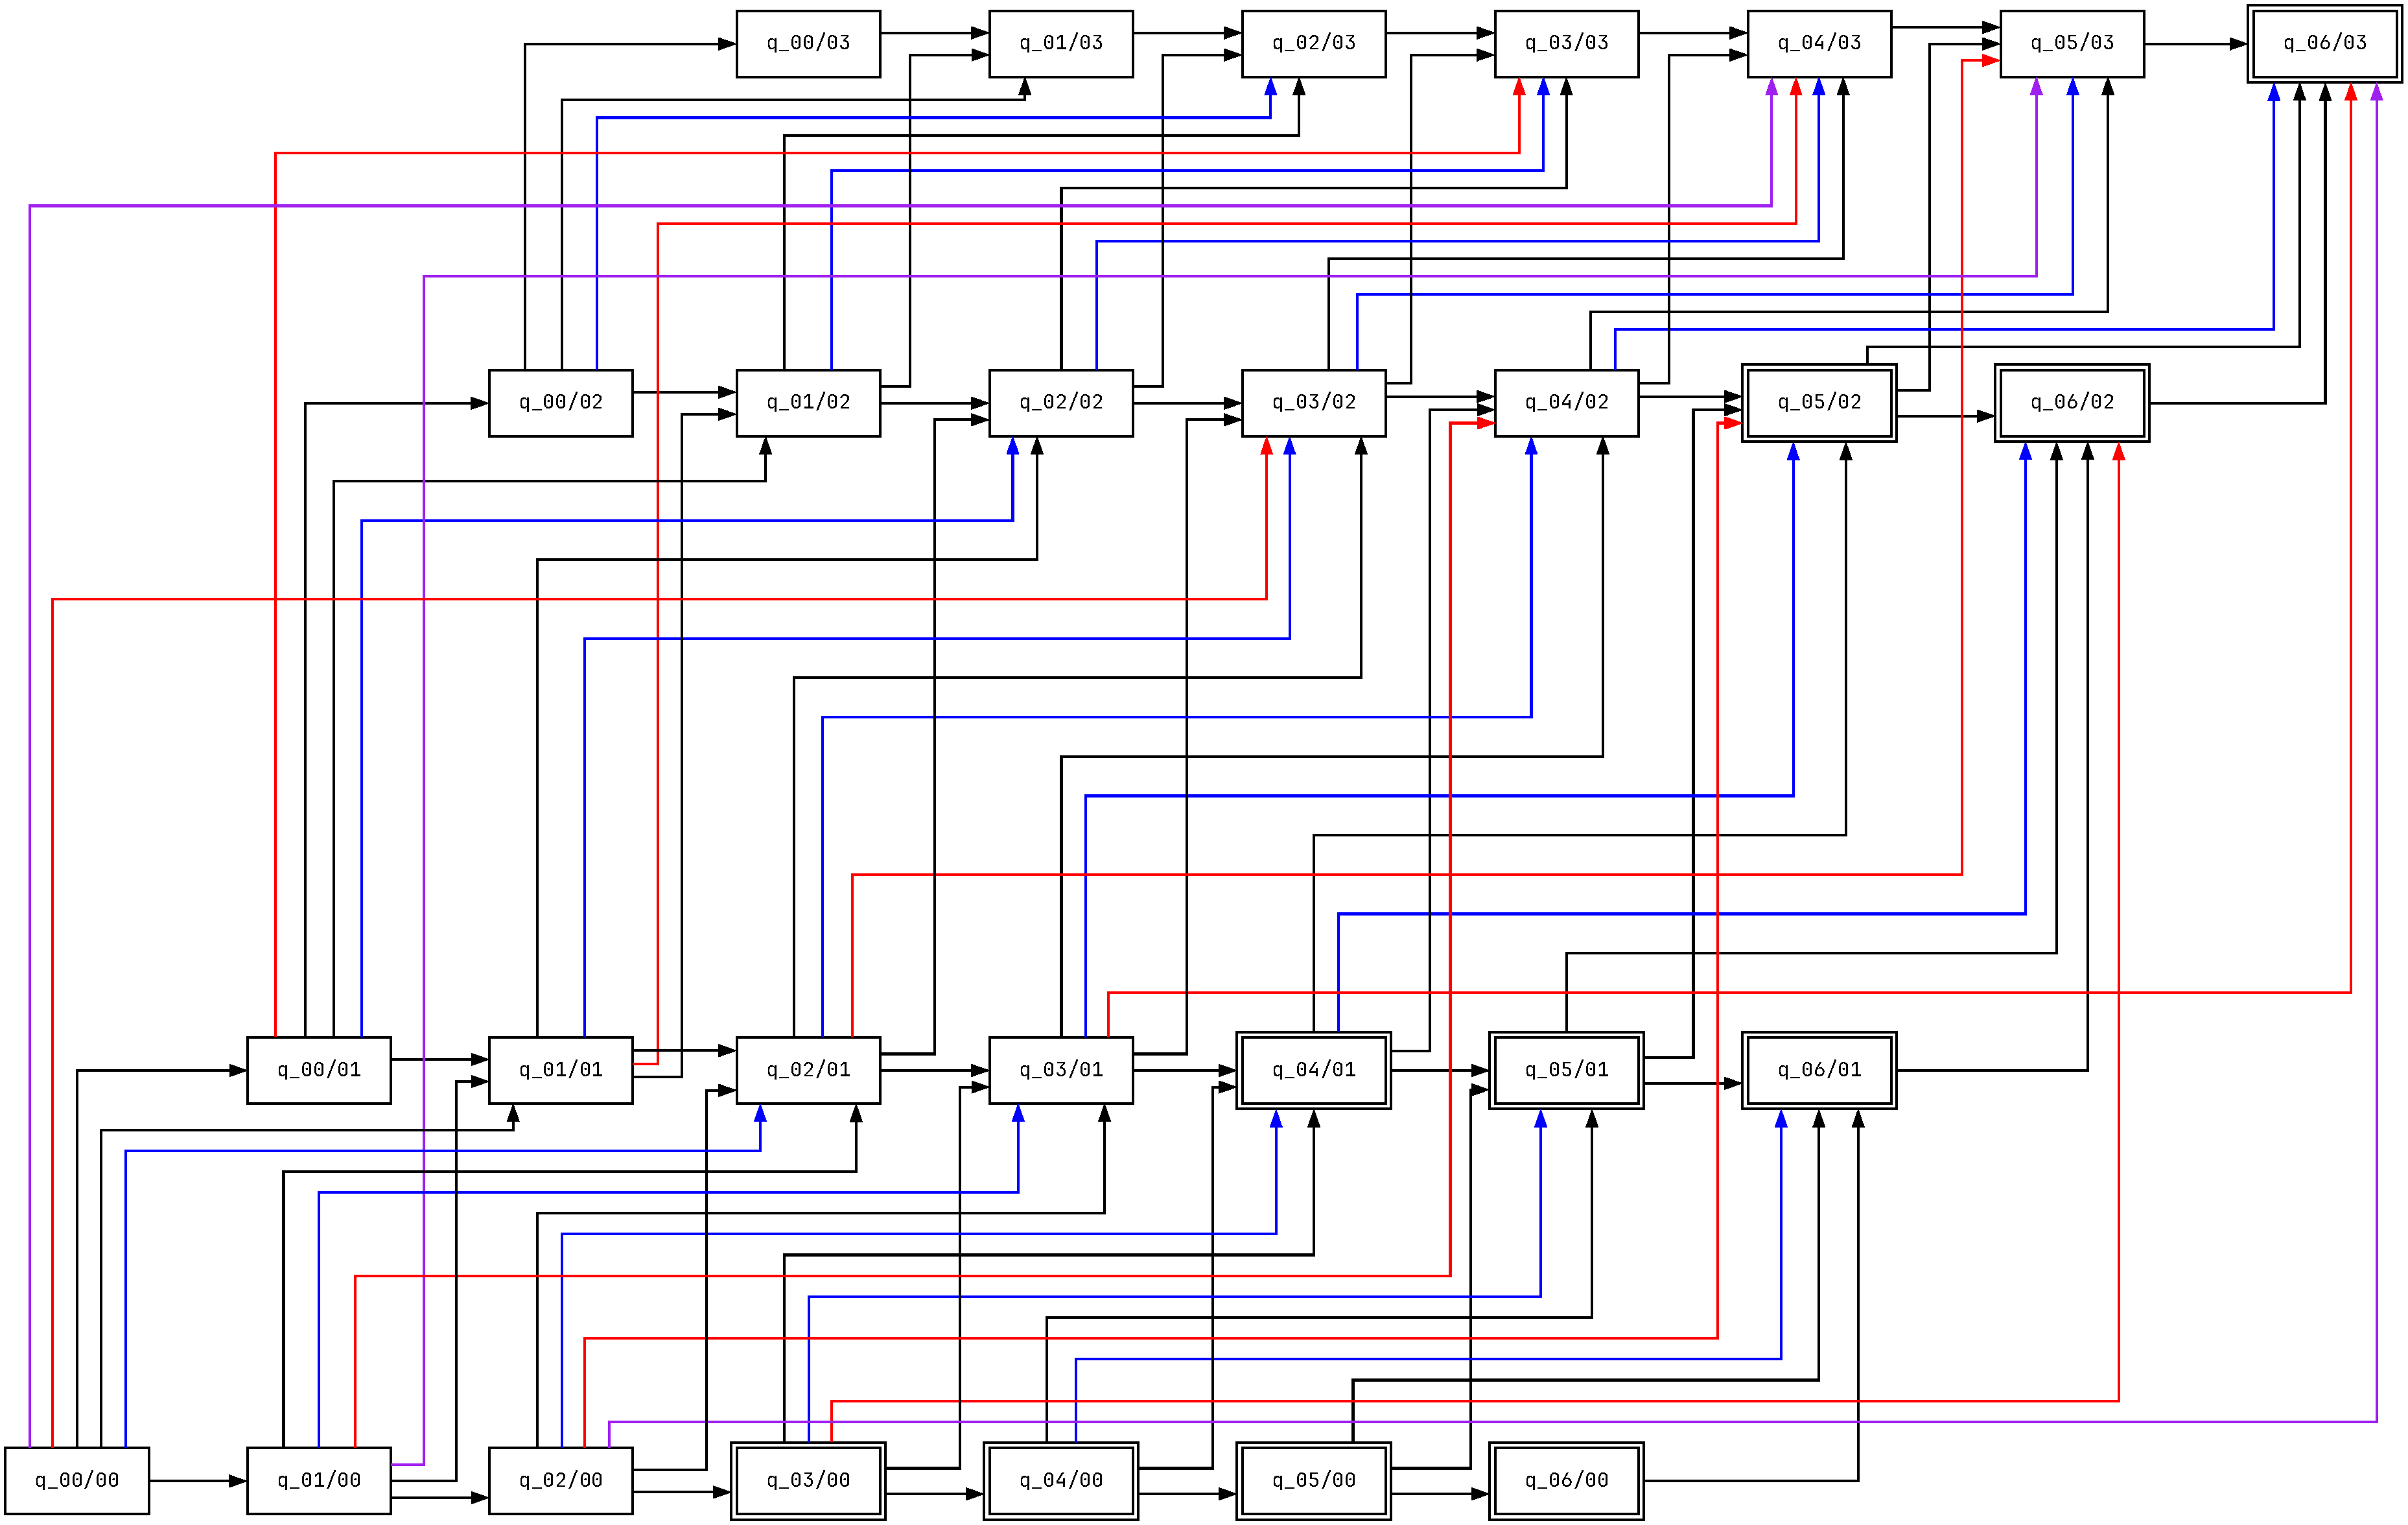
\includegraphics[width=4cm]{figures/lev_nfa_6x3.pdf}}
\adjustbox{valign=m}{\resizebox{0.4\textwidth}{!}{\input{figures/lev_nfa_6x3}}}
\end{center}
\caption{Lev(|\sigma|=6, \Delta=3) automaton, adjacency and reachability matrix.}
\end{figure}

\begin{figure}[H]
\begin{center}
\adjustbox{valign=m}{
\includegraphics[height=4cm]{figures/lev_nfa_6x4.pdf}}
\adjustbox{valign=m}{\resizebox{0.4\textwidth}{!}{\input{figures/lev_nfa_6x4}}}
\end{center}
\caption{Lev(|\sigma|=6, \Delta=4) automaton, adjacency and reachability matrix.}
\end{figure}
\ifSubfilesClassLoaded{\par\clearpage\bibliography{../bib/acmart}}{}
\end{document}
